



\documentclass[12pt,a5paper,openany]{memoir}
\setheadfoot{0pt}{0pt}
\setlrmarginsandblock{2cm}{2cm}{*}
\setulmarginsandblock{.75cm}{1cm}{*}
\checkandfixthelayout
\raggedbottom

\usepackage{fontspec}
\usepackage{titlesec}
\usepackage{xcolor}
\usepackage{enumitem}
\usepackage[defaultlines=5,all]{nowidow}
\usepackage[pdfusetitle,colorlinks=true]{hyperref}
\usepackage{float}
\usepackage{graphicx}
\usepackage{wrapfig}

%% Page style
\makepagestyle{songs}
\makeoddfoot{songs}{}{}{\thepage}
\makeevenfoot{songs}{\thepage}{}{}
% Patch cleardoublepage to not get blank pages after title & contents pages:
\renewcommand\cleardoublepage{\clearpage}
% Suppress page numbers in the toc/frontmatter:
\aliaspagestyle{chapter}{empty}

%% Fonts
\setmainfont[Ligatures=TeX]{DejaVu Sans}

%% Spacings
\setlength{\parindent}{0pt}
\setlength{\tabcolsep}{0pt}
\setlength{\parskip}{1mm}

%% ToC style
% Hide the title of the ToC:
\renewcommand\tocheadstart{}
\renewcommand\printtoctitle[1]{}
\renewcommand\aftertoctitle{}
% Hide section numbers in the ToC:
\renewcommand\numberline[1]{}
\renewcommand\cftdotsep{1}

%% Hyperlinks setup
\hypersetup{
  bookmarks=true,
  linkcolor=.,
  urlcolor=blue,
  pdfcreator=bard v. 1.0.0-rc1 - https://github.com/vojtechkral/bard,
}

%% Song title and subtitle formats
\titleformat{\section}
  {\centering\large\bfseries}{}{0pt}{\underline}
\titlespacing*{\section}
  {0pt}{0pt}{.25ex}
\newcommand\songtitle[1]{%
  % This is a trick to only layout a song on the current page
  % if it fits, otherwise a pagebreak is inserted
  \FloatBlock
  \vfil
  \pagebreak[2]
  \vfilneg
  \section{#1}
}
\newcommand\subtitle[1]{%
  \emph{#1}
}

%% Verse and Chord layout commands
\makeatletter
% The verse & label layout code was written by Jonathan P. Spratte
% under the Beerware license: As long as you retain this notice you
% can do whatever you want with this stuff. If we meet some day, and you think
% this stuff is worth it, you can buy me a beer in return. Jonathan P. Spratte
\newlength\verse@indent
\newlength\verse@labelsep
\newlength\verse@vskip
\AtBeginDocument{% setting AtBeginDocument since earlier we can't rely on em being correct
  \verse@indent=12mm
  \verse@labelsep=2mm
  \verse@vskip=\smallskipamount
}
\newcommand\Verse[1]{%
    \par
    \vskip\verse@vskip
    \noindent\kern-\verse@indent
    \sbox0{\textbf{\footnotesize{#1}}}%
    \ifdim\wd0>\dimexpr\verse@indent-\verse@labelsep\relax
      \usebox0\kern\verse@labelsep
    \else
      \makebox[\verse@indent][l]{\usebox0}%
    \fi
    \ignorespaces
}

\newcommand{\Chord}{\@ifstar{\@Chordalt}{\@Chord}}
\newcommand{\@Chord}[2]{%
  \begin{tabular}[b]{l}%
    \textbf{\textcolor{red}{#1}}\\%  % The chord
    #2\mbox{}\end{tabular}%          % The lyrics
}
\newcommand{\@Chordalt}[3]{%
  \begin{tabular}[b]{l}%
    \textbf{\textcolor{red}{#1}}\\%  % The chord
    \textbf{\textcolor{blue}{#2}}\\% % The alt chord
    #3\mbox{}\end{tabular}%          % The lyrics
}
\makeatother






























% Metadata
\title{Bard Songbook}

% Document
\begin{document}

%% Title page
\frontmatter
\begin{titlingpage}
  \begin{vplace}[0.5]
    \begin{center}
      \Huge{\textbf{Bard Songbook}} \\
      \vspace{0.5cm}
      \LARGE{An example project} \\
        \vspace{1cm}
        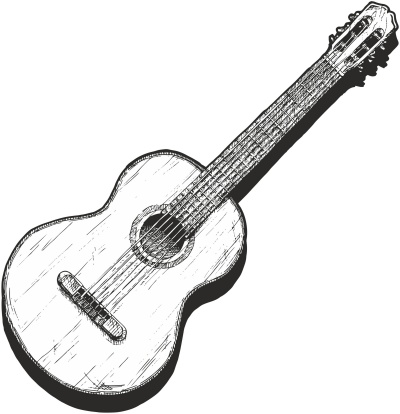
\includegraphics[width=70.55555555555554mm]{guitar.jpg}
      
    \end{center}
  \end{vplace}

  \mbox{}
  \vfill
  \begin{center}\small{A set of a few non-copyrighted songs.}\end{center}
\end{titlingpage}

%% Contents page
\tableofcontents*

%% Songs
\mainmatter

\pagestyle{songs}

  %% song 0
  \songtitle{Danny Boy}

  \begin{center}
      \subtitle{English ballad}
    \end{center}
  
  

  
  \Verse{1.} \Chord{G7}{Oh~Danny~}\Chord{C}{Boy,~the~pipes,~the~}\Chord{C7}{pipes~are~}\Chord{F}{calling}\\
From~glen~to~\Chord{C}{glen,~and~}\Chord{Em}{down~the~}\Chord{F}{mountain~}\Chord{G7}{side}\\
The~summer’s~\Chord{C}{gone,~and~all~the~}\Chord{C7}{flowers~are~}\Chord{F}{dying}\\
‘Tis~you,~’tis~\Chord{C}{you~must~}\Chord{Dm}{go~and~}\Chord{G7}{I~must~}\Chord{C}{bide.}

    \vspace{\parskip}

  
\Verse{Ch1.} \Chord{G7}{But~come~ye~}\Chord{Am}{back~when~}\Chord{F}{summer’s~}\Chord{G7}{in~the~}\Chord{C}{meadow}\\
Or~when~the~\Chord{Am}{valley’s~}\Chord{F}{hushed~and~}\Chord{Em}{white~with~}\Chord{D7}{snow~}\Chord{G7}{}\\
‘Tis~I’ll~be~\Chord{C}{here~in~}\Chord{F}{sunshine~or~in~}\Chord{C}{sha}\Chord{Am}{dow.}\\
Oh~Danny~\Chord{C}{Boy,~oh~Danny~}\Chord{F}{Boy,~I~}\Chord{G7}{love~you~}\Chord{C}{so.}

    \vspace{\parskip}

  
\Verse{2.} And~if~you~come,~when~all~the~flowers~are~dying\\
And~I~am~dead,~as~dead~I~well~may~be\\
You’ll~come~and~find~the~place~where~I~am~lying\\
And~kneel~and~say~an~”Ave”~~there~for~me.

    \vspace{\parskip}

  
\Verse{Ch2.} And~I~shall~hear,~though~soft~you~tread~above~me\\
And~all~my~dreams~will~warm~and~sweeter~be\\
If~you’ll~not~fail~to~tell~me~that~you~love~me\\
I’ll~sleep~in~peace~until~you~come~to~me.

    \vspace{\parskip}

   

    \begin{figure}[H]
      \centering
      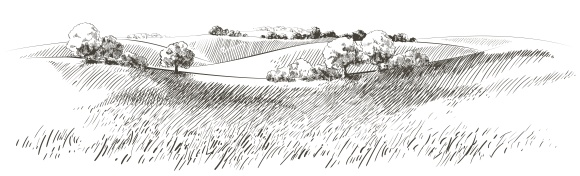
\includegraphics[width=102.30555555555554mm]{hills.jpg}
    \end{figure}

  

    \vspace{\parskip}

  


  %% song 1
  \songtitle{Handsome Molly}

  \begin{center}
      \subtitle{U.S. Old-time}
    \end{center}
  
  

  
  \Verse{1.} \Chord{G}{I~wish~I~was~in~London}\\
Or~some~other~seaport~\Chord{D}{town}\\
\Chord{D}{I'd~step~my~foot~on~a~steamboat}\\
And~sail~the~ocean~\Chord{G}{round}

    \vspace{\parskip}

  
\Verse{2.} While~sailing~round~the~ocean\\
While~sailing~round~the~sea\\
I’d~think~of~Handsome~Molly\\
Wherever~she~may~be

    \vspace{\parskip}

  
\Verse{3.} I~went~to~church~last~Sunday\\
She~passed~me~on~by\\
I~knew~her~mind~was~changing\\
By~the~roving~of~her~eye

    \vspace{\parskip}

  
\Verse{4.} Her~hair~as~black~as~a~Raven’s\\
Her~eyes~were~black~as~coal\\
Her~teeth~just~like~lilies\\
Out~in~the~morning~cold

    \vspace{\parskip}

  
\Verse{5.} Now~do~you~remember~Molly\\
When~you~gave~me~your~right~hand\\
Said~if~you~ever~married\\
Then~I’d~be~the~man

    \vspace{\parskip}

  
\Verse{6.} Now~you’ve~broke~your~promise\\
Go~marry~whom~you~please\\
My~heart~is~broken\\
‘Til~I~get~some~ease

    \vspace{\parskip}

  


  %% song 2
  \songtitle{Whiskey in the Jar}

  \begin{center}
      \subtitle{Irish traditional}
    \end{center}
  
  

  
  \Verse{1.} As~\Chord{C}{I~was~a~goin'~over}\\
The~\Chord{Am}{far~famed~Kerry~mountains}\\
I~\Chord{F}{met~with~Captain~Farrell~and~his}\\
\Chord{C}{Money~he~was~counting}\\
\Chord{C}{I~first~produced~my~pistol}\\
And~I~\Chord{Am}{~then~produced~my~rapier}\\
Saying~\Chord{F}{~"Stand~and~deliver,}\\
For~\Chord{C}{you~are~a~bold~deceiver!"}

    \vspace{\parskip}

  
\Verse{Ch.} Mush-a~\Chord{G}{ring~dum-a~do~dum-a~da}\\
\Chord{C}{Whack~for~me~daddy-o}\\
\Chord{F}{Whack~for~me~daddy-o}\\
There's~\Chord{C}{whiskey~}\Chord{G}{in~the~}\Chord{C}{jar}

    \vspace{\parskip}

  
\Verse{2.} I~counted~out~his~money\\
And~it~made~a~pretty~penny\\
I~put~it~in~me~pocket\\
And~I~took~it~home~to~Jenny\\
She~sighed~and~she~swore\\
That~she~never~would~deceive~me\\
But~the~devil~take~the~women\\
For~they~never~can~be~easy\\
\emph{Ch.}

    \vspace{\parskip}

  
\Verse{3.} I~went~up~to~my~chamber\\
All~for~to~take~a~slumber\\
I~dreamt~of~gold~and~jewels\\
And~for~sure~'t~was~no~wonder\\
But~Jenny~drew~me~charges\\
And~she~filled~them~up~with~water\\
Then~sent~for~captain~Farrell\\
To~be~ready~for~the~slaughter\\
\emph{Ch.}

    \vspace{\parskip}

  
\Verse{4.} 'Twas~early~in~the~morning\\
Just~before~I~rose~to~travel\\
Up~comes~a~band~of~footmen\\
And~likewise~captain~Farrell\\
I~first~produced~me~pistol\\
For~she~stole~away~me~rapier\\
I~couldn't~shoot~the~water\\
So~a~prisoner~I~was~taken\\
\emph{Ch.}

    \vspace{\parskip}

   

    \begin{figure}[H]
      \centering
      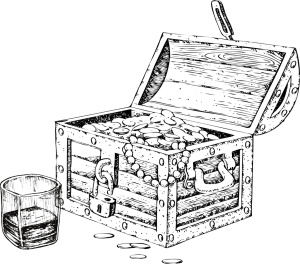
\includegraphics[width=52.916666666666664mm]{chest.jpg}
    \end{figure}

  

    \vspace{\parskip}

  


  %% song 3
  \songtitle{Wild Mountain Thyme}

  \begin{center}
      \subtitle{Irish \& Scottish traditional}
    \end{center}
  
  

  
  \Verse{1.} O'~the~\Chord{G}{summer~}\Chord{C}{time~}\Chord{G}{has~come}\\
And~the~\Chord{C}{trees~are~sweetly~}\Chord{G}{bloomin'}\\
And~the~\Chord{C}{wild~}\Chord{G}{mountain~}\Chord{Em}{thyme}\\
Grows~\Chord{C}{around~the~}\Chord{Am}{bloomin'~}\Chord{C}{heather}\\
Will~ye~\Chord{G}{go~}\Chord{C}{lassie~}\Chord{G}{go?}

    \vspace{\parskip}

  
\Verse{Ch.} And~we'll~\Chord{C}{all~go~}\Chord{G}{together~to~pull~}\Chord{C}{wild~}\Chord{G}{mountain~}\Chord{Em}{thyme}\\
All~\Chord{C}{around~the~}\Chord{Am}{bloomin'~}\Chord{C}{heather,~will~ye~}\Chord{G}{go~}\Chord{C}{lassie~}\Chord{G}{go?}

    \vspace{\parskip}

  
\Verse{2.} I~will~build~my~love~a~bower\\
By~yon~cool~crystal~fountain~
    \hfill\hspace{0pt}\vspace{-1em}
    \begin{wrapfigure}{r}{26.458333333333332mm}
      \centering
      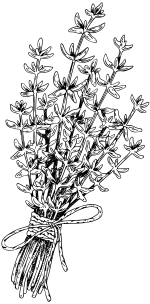
\includegraphics[width=26.458333333333332mm]{thyme.png}
    \end{wrapfigure}
  \\
And~round~it~I~will~pile\\
All~the~wild~flowers~o'~the~mountain.\\
Will~ye~go~lassie~go? \emph{Ch.}

    \vspace{\parskip}

  
\Verse{3.} I~will~range~through~the~wilds\\
And~the~deep~glen~sae~dreamy\\
And~return~wi'~their~spoils\\
Tae~the~bower~o'~my~dearie.\\
Will~ye~go~lassie~go? \emph{Ch.}

    \vspace{\parskip}

  
\Verse{4.} If~my~true~love~she'll~not~come\\
Then~I'll~surely~find~another\\
To~pull~wild~mountain~thyme\\
All~around~the~bloomin'~heather.\\
Will~ye~go~lassie~go? \emph{Ch.}

    \vspace{\parskip}

  



\backmatter
\pagestyle{empty}



\end{document}
